\begin{tikzpicture}[scale=0.9,transform shape] 
	\onslide<1->{ \node[] (input_taj) 
		{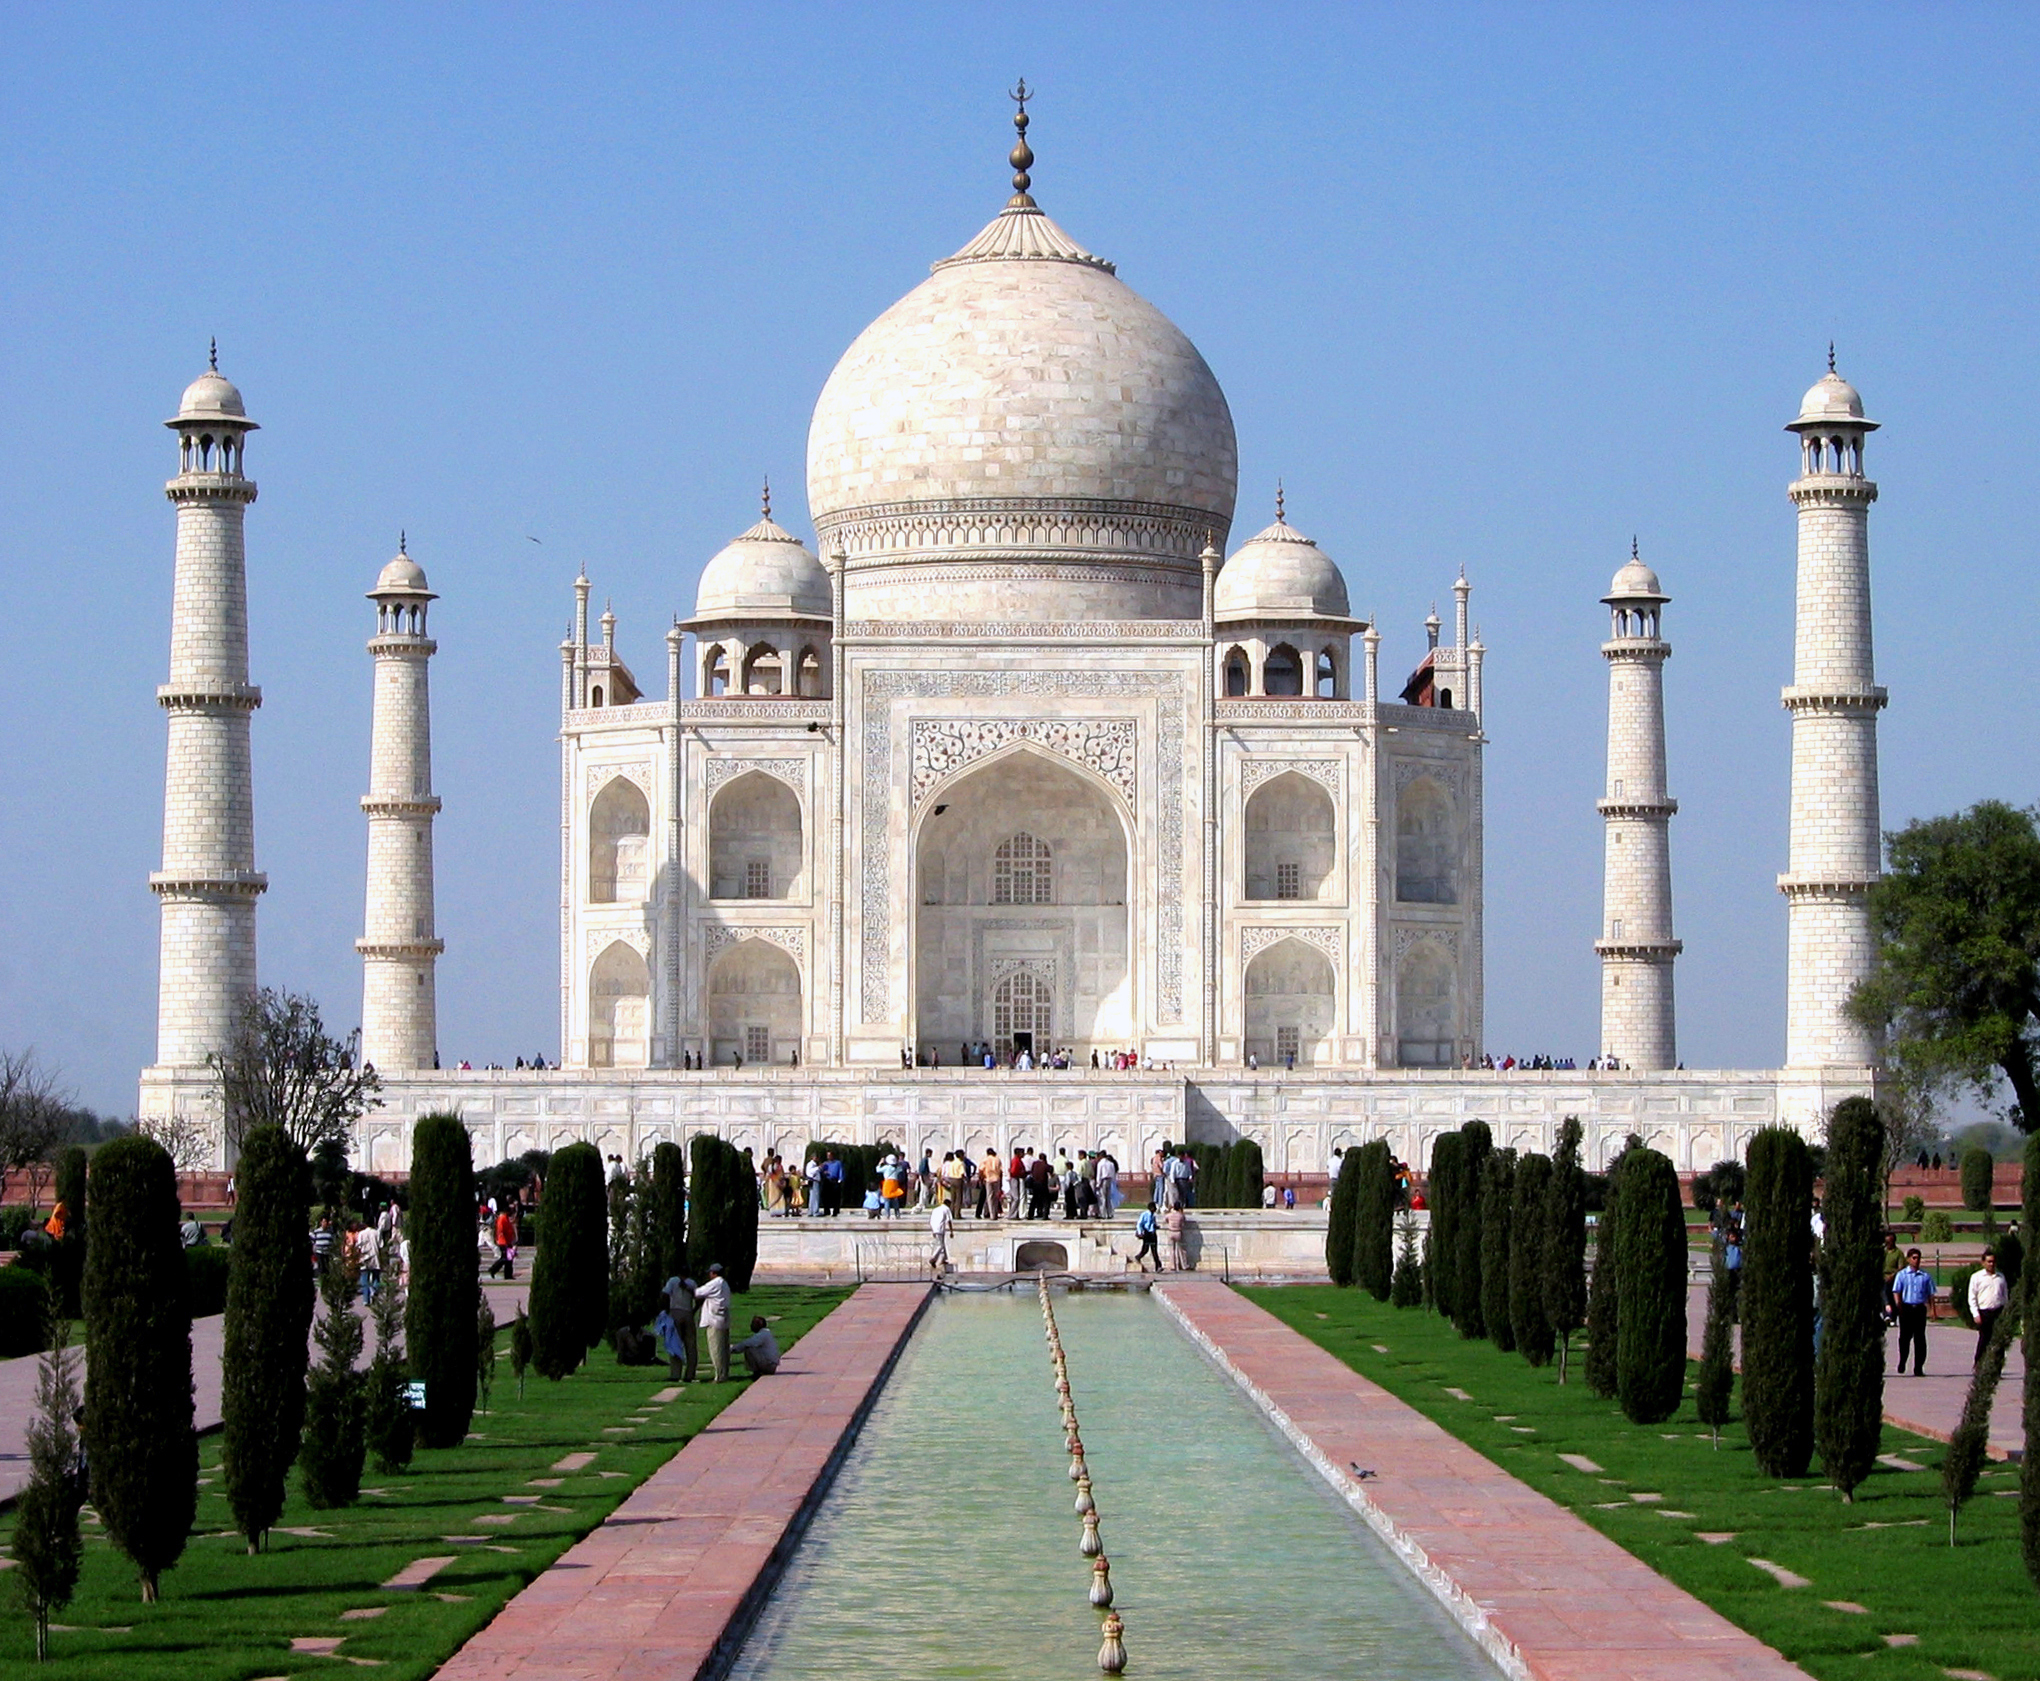
\includegraphics[width=20mm,scale=0.7]{images/taj_mahal.jpg}};
	}
	\onslide<1->{  \node [right=3cm of input_taj.south,anchor=south west] (raw)  { 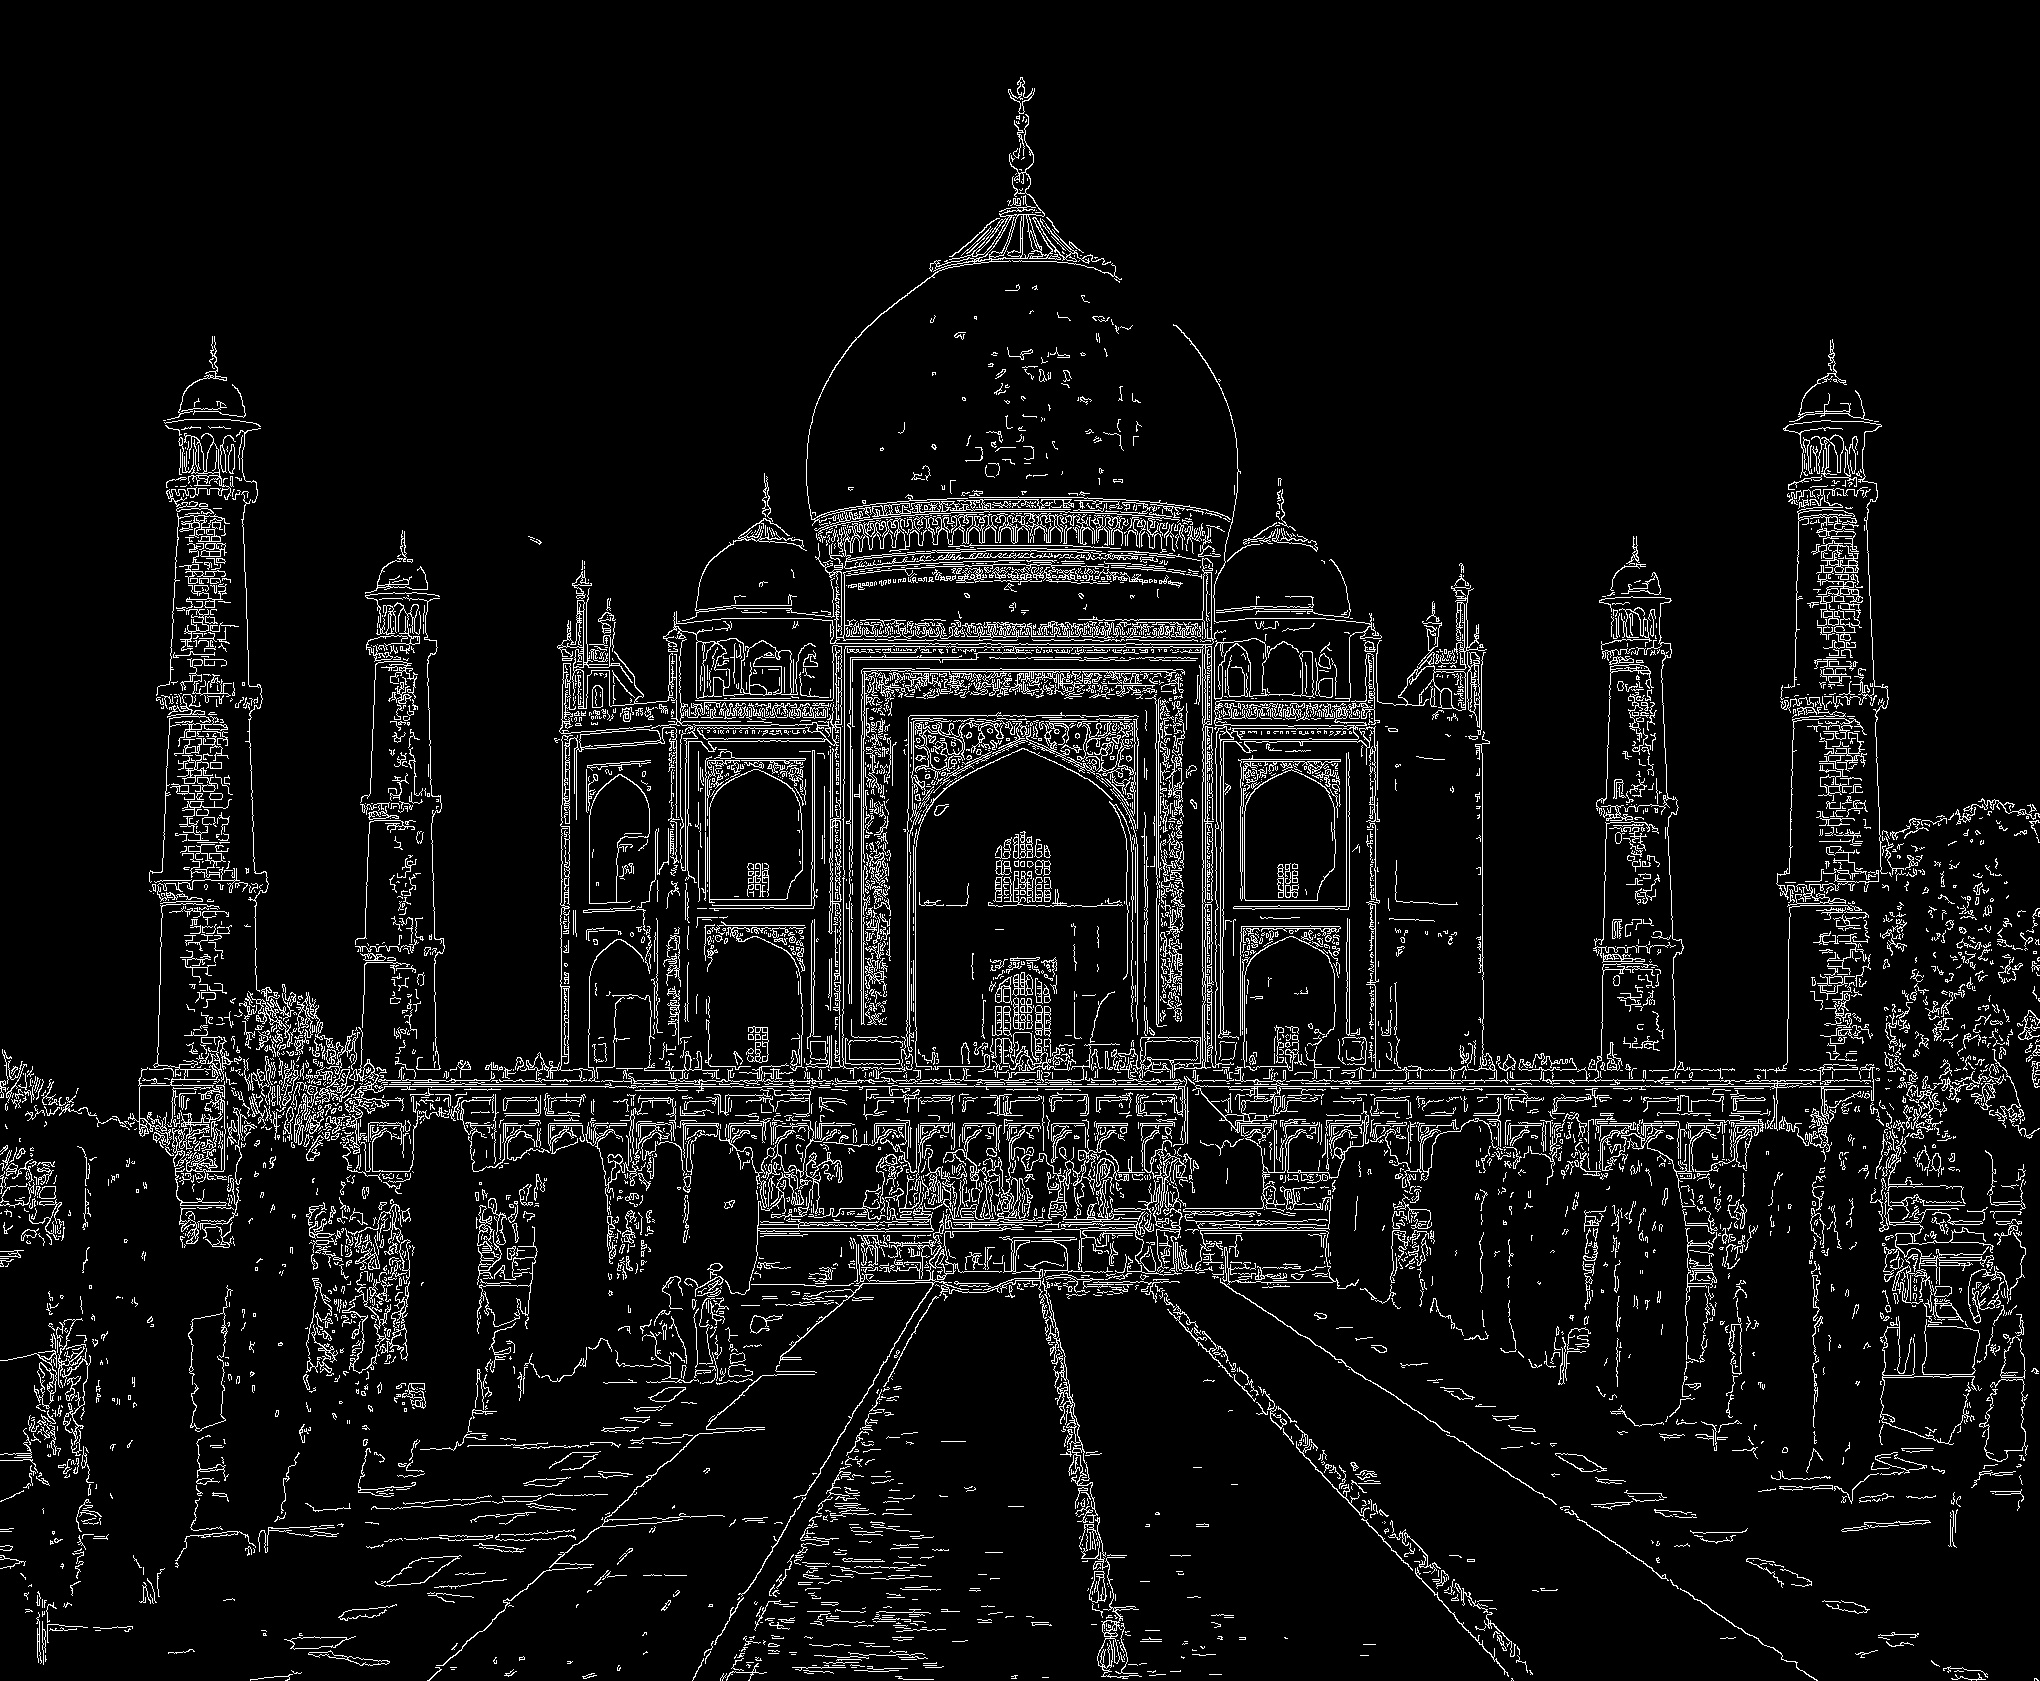
\includegraphics[width=20mm,scale=0.7]{images/taj_mahal_detectedges.jpg}};
		\node [below of = raw,anchor=north] (edge)  { \resizebox{15mm}{5mm}{ \begin{tabular}{ccccc}
			0 & 0  & 0  & 0  & 0   \\
			0 & 1 & 1 & 1  & 0   \\
			0 & 1 & -8  & 1 & 0  \\
			0 & 1  & 1 & 1  & 0   \\
			0 & 0  & 0  & 0  & 0  
			\end{tabular} }};
		\node[above of= raw,node distance=1.2cm ] (features)  {\footnotesize{Features}};
		\draw[->,thick] (input_taj) -- (raw) ;

	}
	\onslide<1->{\node [right=5cm of raw.center,anchor= center](output_taj){car, bus, \textcolor{blue}{monument}, flower};
		\draw[->,thick] (raw) -- (output_taj) ;
		\node [] (o) at ($(output_taj) + (0,1.2)$) {\footnotesize{Classifier}};
		\node [] (i) at ($(input_taj) + (0,1.2)$) {\footnotesize{Input}};
	}

\end{tikzpicture}